\chapter{Design patterns}

`Choose two design patterns among those that we saw in class,4
and that you did not use in the 3rd assignment.
For each chosen design pattern, you must have a corresponding implementation in your code. If not,
refactor your code to include it.'

\section{Model View Controller}

\subsection{MVC Description}
The MVC is implemented by using JavaFX. If you look at the figure below, you see the principle of the MVC design pattern. The model is loaded by creating a Stage with a FXML file as resource. This model in turn creates the view and a controller. All further handling of the view is done in the controller. 
\\
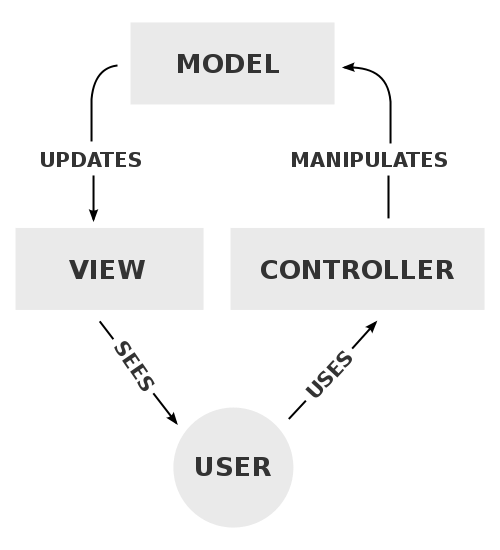
\includegraphics[width=100mm]{MVC.png}

\subsection{MVC Class Diagram}

Below is the class diagram of the Model View Controller design pattern, found in our code.
\\
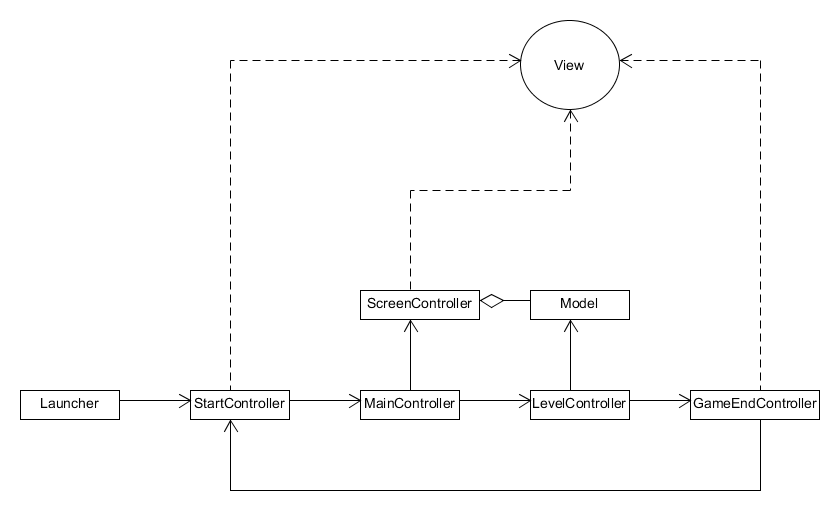
\includegraphics[width=100mm]{UML_MVC.png}

\subsection{MVC Sequence Diagram}
`Make a sequence diagram of how the pattern works dynamically in your code'